% This file was created with tikzplotlib v0.9.17.
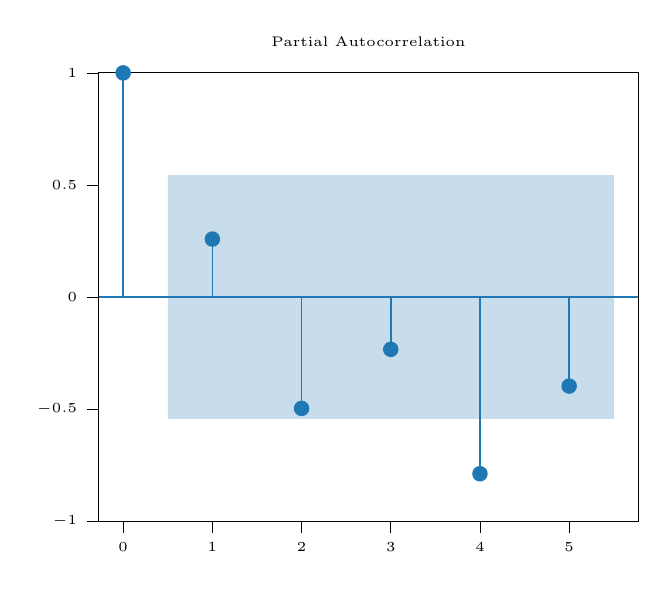
\begin{tikzpicture}

\definecolor{color0}{rgb}{0.12156862745098,0.466666666666667,0.705882352941177}

\begin{axis}[
font={\fontsize{3}{12}\selectfont},
tick align=outside,
tick pos=left,
title={Partial Autocorrelation},
x grid style={white!69.0196078431373!black},
xmin=-0.275, xmax=5.775,
xtick style={color=black},
y grid style={white!69.0196078431373!black},
ymin=-1, ymax=1,
ytick style={color=black}
]
\path [fill=color0, fill opacity=0.25]
(axis cs:0.5,0.543596203409375)
--(axis cs:0.5,-0.543596203409375)
--(axis cs:2,-0.543596203409375)
--(axis cs:3,-0.543596203409375)
--(axis cs:4,-0.543596203409375)
--(axis cs:5.5,-0.543596203409375)
--(axis cs:5.5,0.543596203409375)
--(axis cs:5.5,0.543596203409375)
--(axis cs:4,0.543596203409375)
--(axis cs:3,0.543596203409375)
--(axis cs:2,0.543596203409375)
--(axis cs:0.5,0.543596203409375)
--cycle;

\path [draw=color0, semithick]
(axis cs:0,0)
--(axis cs:0,1);

\path [draw=color0, semithick]
(axis cs:1,0)
--(axis cs:1,0.258540805523111);

\path [draw=color0, semithick]
(axis cs:2,0)
--(axis cs:2,-0.496797494225477);

\path [draw=color0, semithick]
(axis cs:3,0)
--(axis cs:3,-0.233353450354527);

\path [draw=color0, semithick]
(axis cs:4,0)
--(axis cs:4,-0.788294461063737);

\path [draw=color0, semithick]
(axis cs:5,0)
--(axis cs:5,-0.39711440531646);

\addplot [semithick, color0]
table {%
-0.275 -2.22044604925031e-16
5.775 -2.22044604925031e-16
};
\addplot [semithick, color0, mark=*, mark size=2.5, mark options={solid}, only marks]
table {%
0 1
1 0.258540805523111
2 -0.496797494225477
3 -0.233353450354527
4 -0.788294461063737
5 -0.39711440531646
};
\end{axis}

\end{tikzpicture}
